\documentclass[a4paper]{article}

%% Language and font encodings
\usepackage[english]{babel}
\usepackage[utf8x]{inputenc}
\usepackage[T1]{fontenc}

%% Sets page size and margins
\usepackage[a4paper,top=3cm,bottom=2cm,left=3cm,right=3cm,marginparwidth=1.75cm]{geometry}

%% Useful packages
\usepackage{amsmath}
\usepackage{graphicx}
\usepackage[colorinlistoftodos]{todonotes}
\usepackage[colorlinks=true, allcolors=blue]{hyperref}
\usepackage{lipsum}
\usepackage{mwe}
\usepackage{subcaption} 



\title{Speaker Diarization: Using Recurrent Neural Networks}
\author{Vishal Sharma, Zekun Zhang, Zachary Neubert}

\begin{document}
\maketitle

\begin{abstract}
Speaker Diarization is the problem of separating speakers in an audio. There could be any number of speakers and final result should state when speaker starts and ends. In this project, we analyze given audio file with 2 channels and 2 speakers (on separate channel). We train Neural Network for learning when a person is speaking. We use different type of Neural Networks specifically, Single Layer Perceptron (SLP), Multi Layer Perceptron (MLP), Recurrent Neural Network (RNN) and Convolution Neural Network (CNN) we achieve  $\sim$92\% of accuracy with RNN. 
\end{abstract}

\section{Introduction}

Speaker diarization is the task of determining "who spoke when?"\cite{anguera2010speaker} in an audio with unknown number of speakers and unknown length of audio. It is of great importance in the domain of speech research and has several applications in the field of information retrieval \cite{anguera2012speaker} \cite{pawelDeepRNN}.

\section{Dataset}
Our dataset contains 37 audio files approximately of 15 minutes each with sampling rate of 44100 samples/second, recorded in 2 channels with exactly 2 speakers on 2 different microphones. Each audio file has been hand annotated for speakers timings. Annotating timing (in seconds) they start and stop speaking. We use this dataset and split in 3 parts for training, validation and testing. 

\section{Preprocessing}

\subsection{Data Normalization}
We perform normalization of audio files after observing recorded audio was not in the same scale. Few audio files were louder than others and normalization can help bring all audio files to same scale.

\subsection{Sampling Audio}
With frame rate being high, we have a lot of data. To give an example, in a 15 min audio file we get about 40M samples in each channel.  To reduce data without loosing much information, we down sample audio files by every 4 sample. \cite{giannakopoulos2015pyaudioanalysis}

\subsection{Cleaning Labels}
Provided labels needed some cleaning described below:
\begin{enumerate}
\item Names of the speakers was not consistent throughout the data file, we cleaned it and made sure name is consistent.
\item File also contained unicode, which needed to be cleaned. Python goes crazy with unicodes lol
\item There were miss alignments as well in the data and needed to be removed and fixed.
\end{enumerate}	

\section{Approach}

\subsection{Multi-layer Perceptron}
We start with a basic single layer perceptron model. We implement 3 different models with hidden layer of different sizes 100, 200, 500 neurons. We achieve approximately 86\% accuracy. 
We next move to multi-layer perceptron model and try models with 2 layers deep. First layer had 100 and second 50 neurons and another with higher number of neurons (First Layer: 200, Second Layer: 100) (First Layer: 300, Second Layer: 50). For all the networks used in this project, the hidden neurons are ReLu \cite{relu} and the output neuron are sigmoid. The cost function used is cross entropy and mini-batch gradient descent with Adam optimization is used to train network.

\subsection{Recurrent Neural Network (RNN)}
Next we try Recurrent Neural Network \cite{mikolov2010recurrent} on the classification problem. The RNN gives us the best result with 3 layers each with 150 Long short-term memory (LSTM) cells. The LSTM in the graph means a LSTM layer which consists of 150 LSTM cells. The output only has one neuron with sigmoid to predict 0 or 1. 

\begin{figure}
\centering
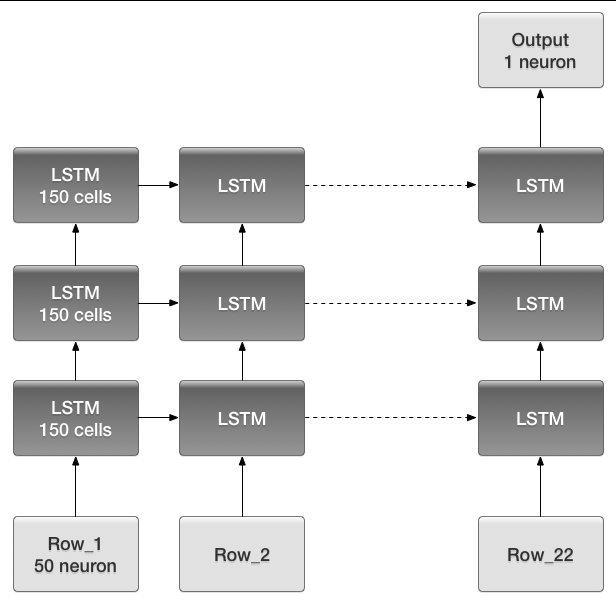
\includegraphics[width=0.8\textwidth]{RNN.png}
\caption{\label{fig:RNN}Structure of RNN using TensorFlow.}
\end{figure}


\subsection{Convolution Neural Network}
To apply CNN \cite{krizhevsky2012imagenet}, we at first compute the spectrogram for each row of the data matrix, then store them into a new file by using pickle. In this way we don’t need to compute spectrogram online and hence can save a lot of training time. Function scipy. signal.spectrogram is used to compute the spectrogram for each segment. The recomputed spectrogram of each segment then is organized to a 3 dimension matrix with shape (number of segments, height, width). For example, the down sampled data matrix of a channel returned by get data has the shape (100, 1102) for a channel with 100 segments, then the shape of recomputed spectrogram matrix is (100,129,4). The number of segments remains the same. The height 129 and width 4 come from using the default parameters of function scipy. signal.spectrogram. Spectrogram matrices are computed and stored by using code in Spectrogram Generator.

\begin{figure}
\centering
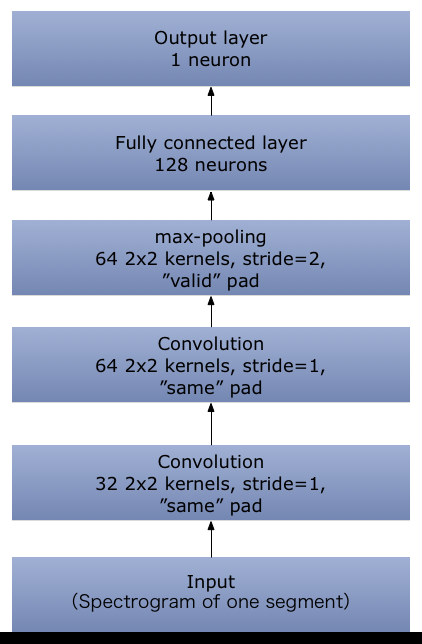
\includegraphics[width=0.5\textwidth]{CNN.png}
\caption{\label{fig:CNN}Structure of CNN using TensorFlow.}
\end{figure}


\begin{figure} 
\centering
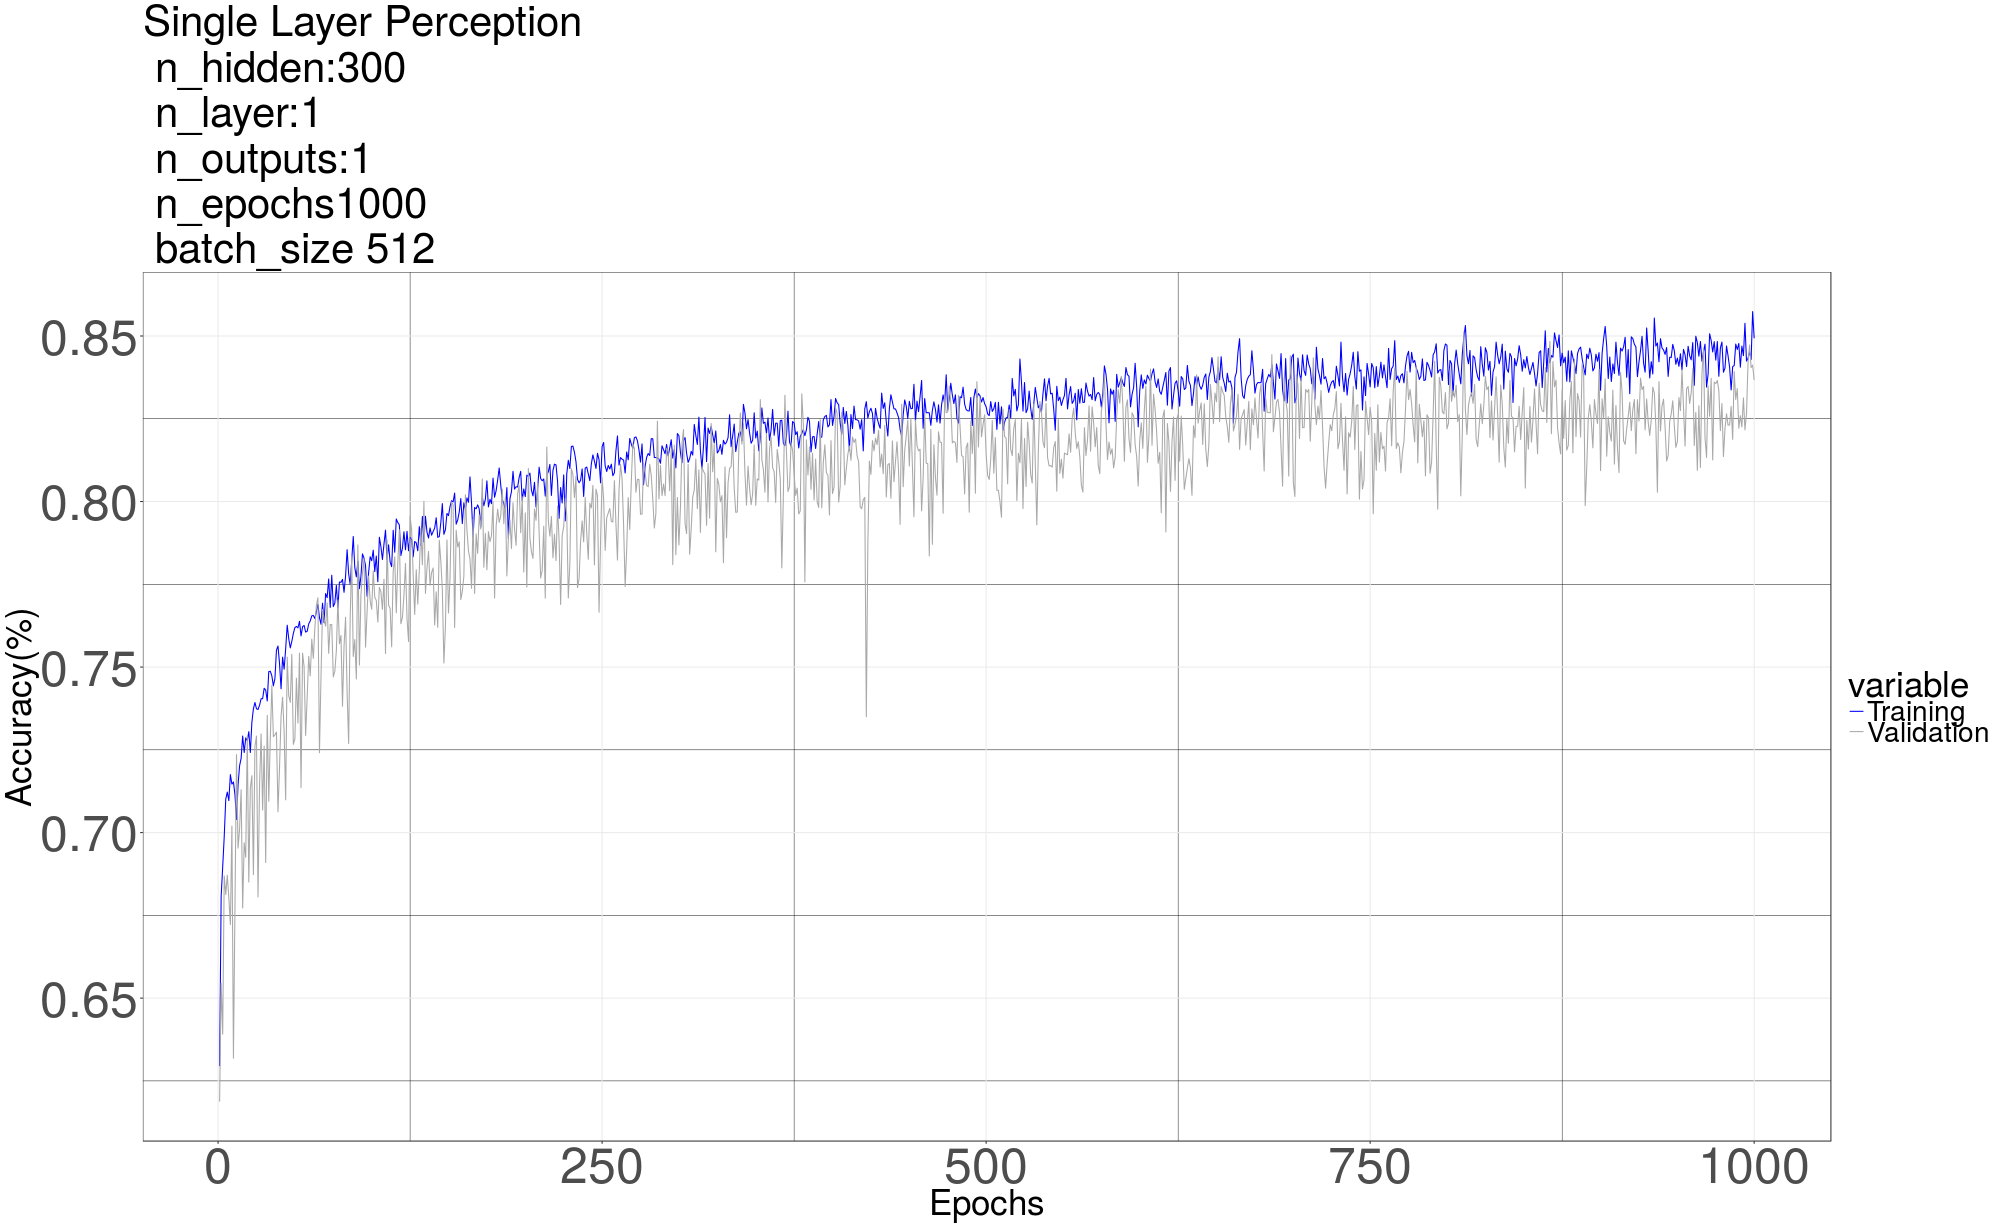
\includegraphics[width=1.0\textwidth]{MLP_2.png}
\caption{\label{fig:MLP_2}Results of Single Layer Perceptron on Training and Validation set. Title contains information about configuration of the network.}
\end{figure}

\begin{figure}  
\centering
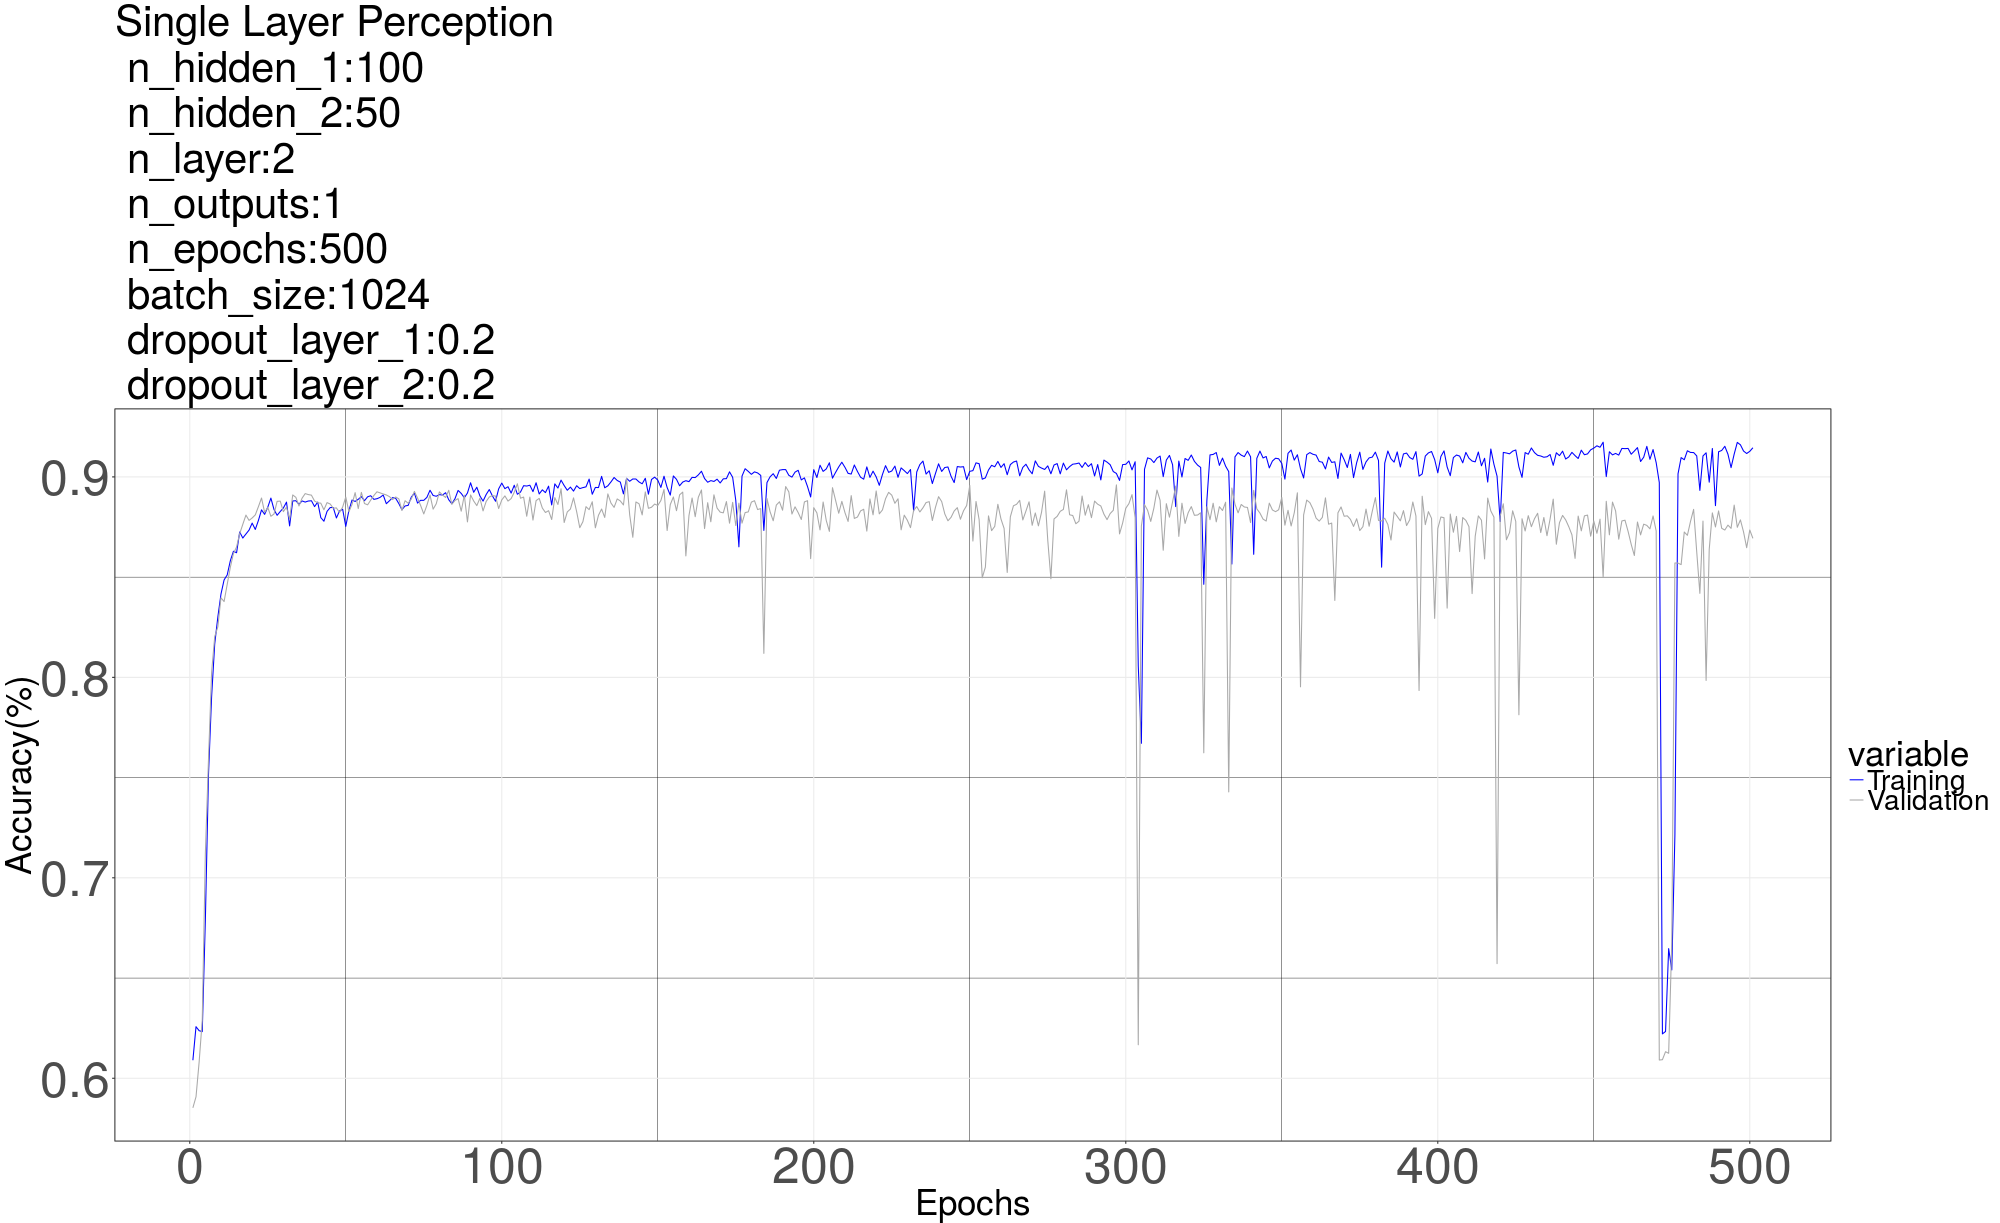
\includegraphics[width=1.0\textwidth]{MLP_6.png}
\caption{\label{fig:MLP_6}Results of Multi Layer Perceptron on Training and Validation set. Title contains information about configuration of the network.}
\end{figure}


\begin{figure}  
\centering
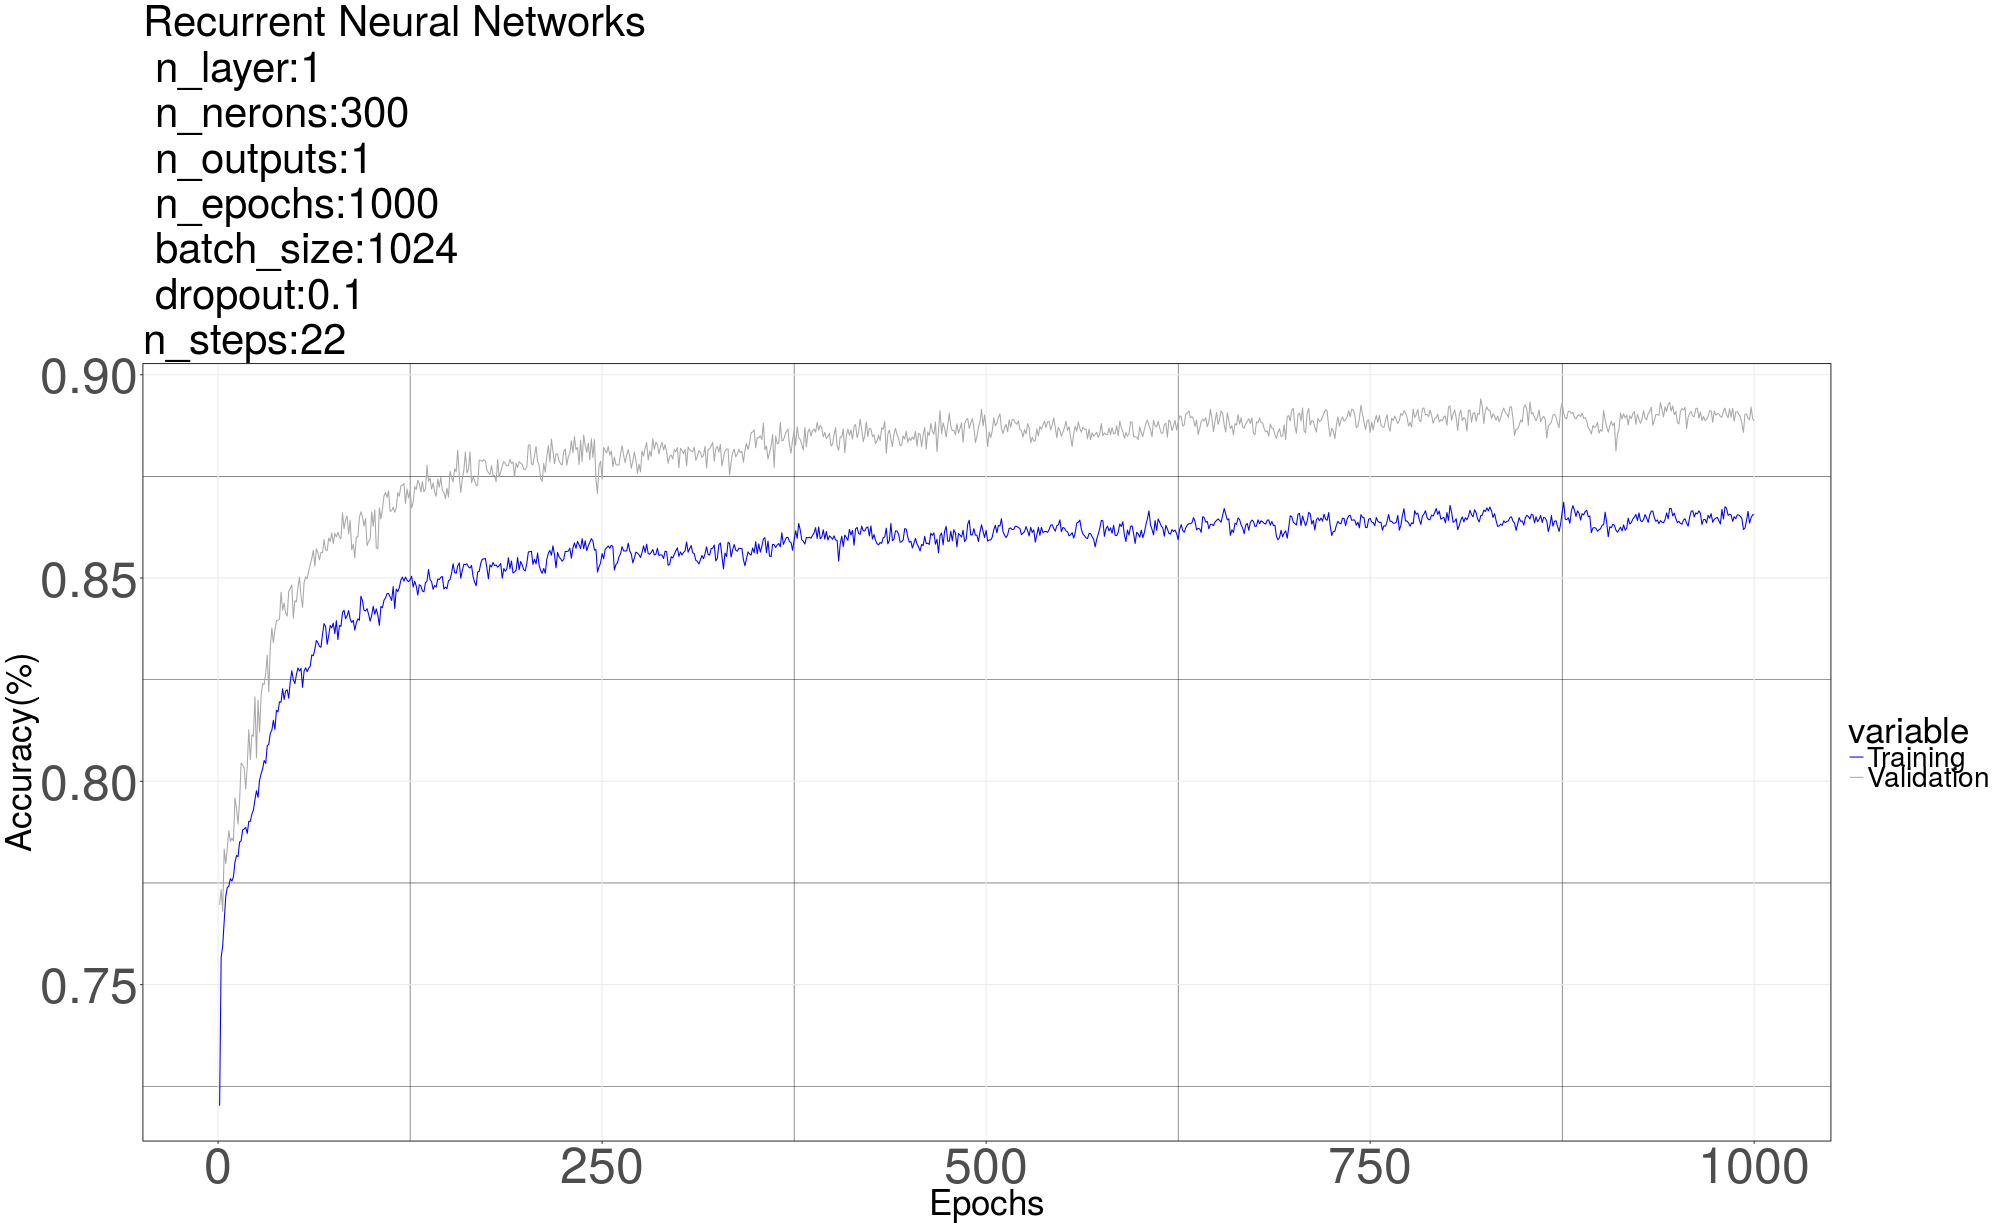
\includegraphics[width=1.0\textwidth]{RNN_1.png}
\caption{\label{fig:RNN_1}Results of Recurrent Neural Network on Training and Validation set. Title contains information about configuration of the network.}
\end{figure}

\begin{figure}  
\centering
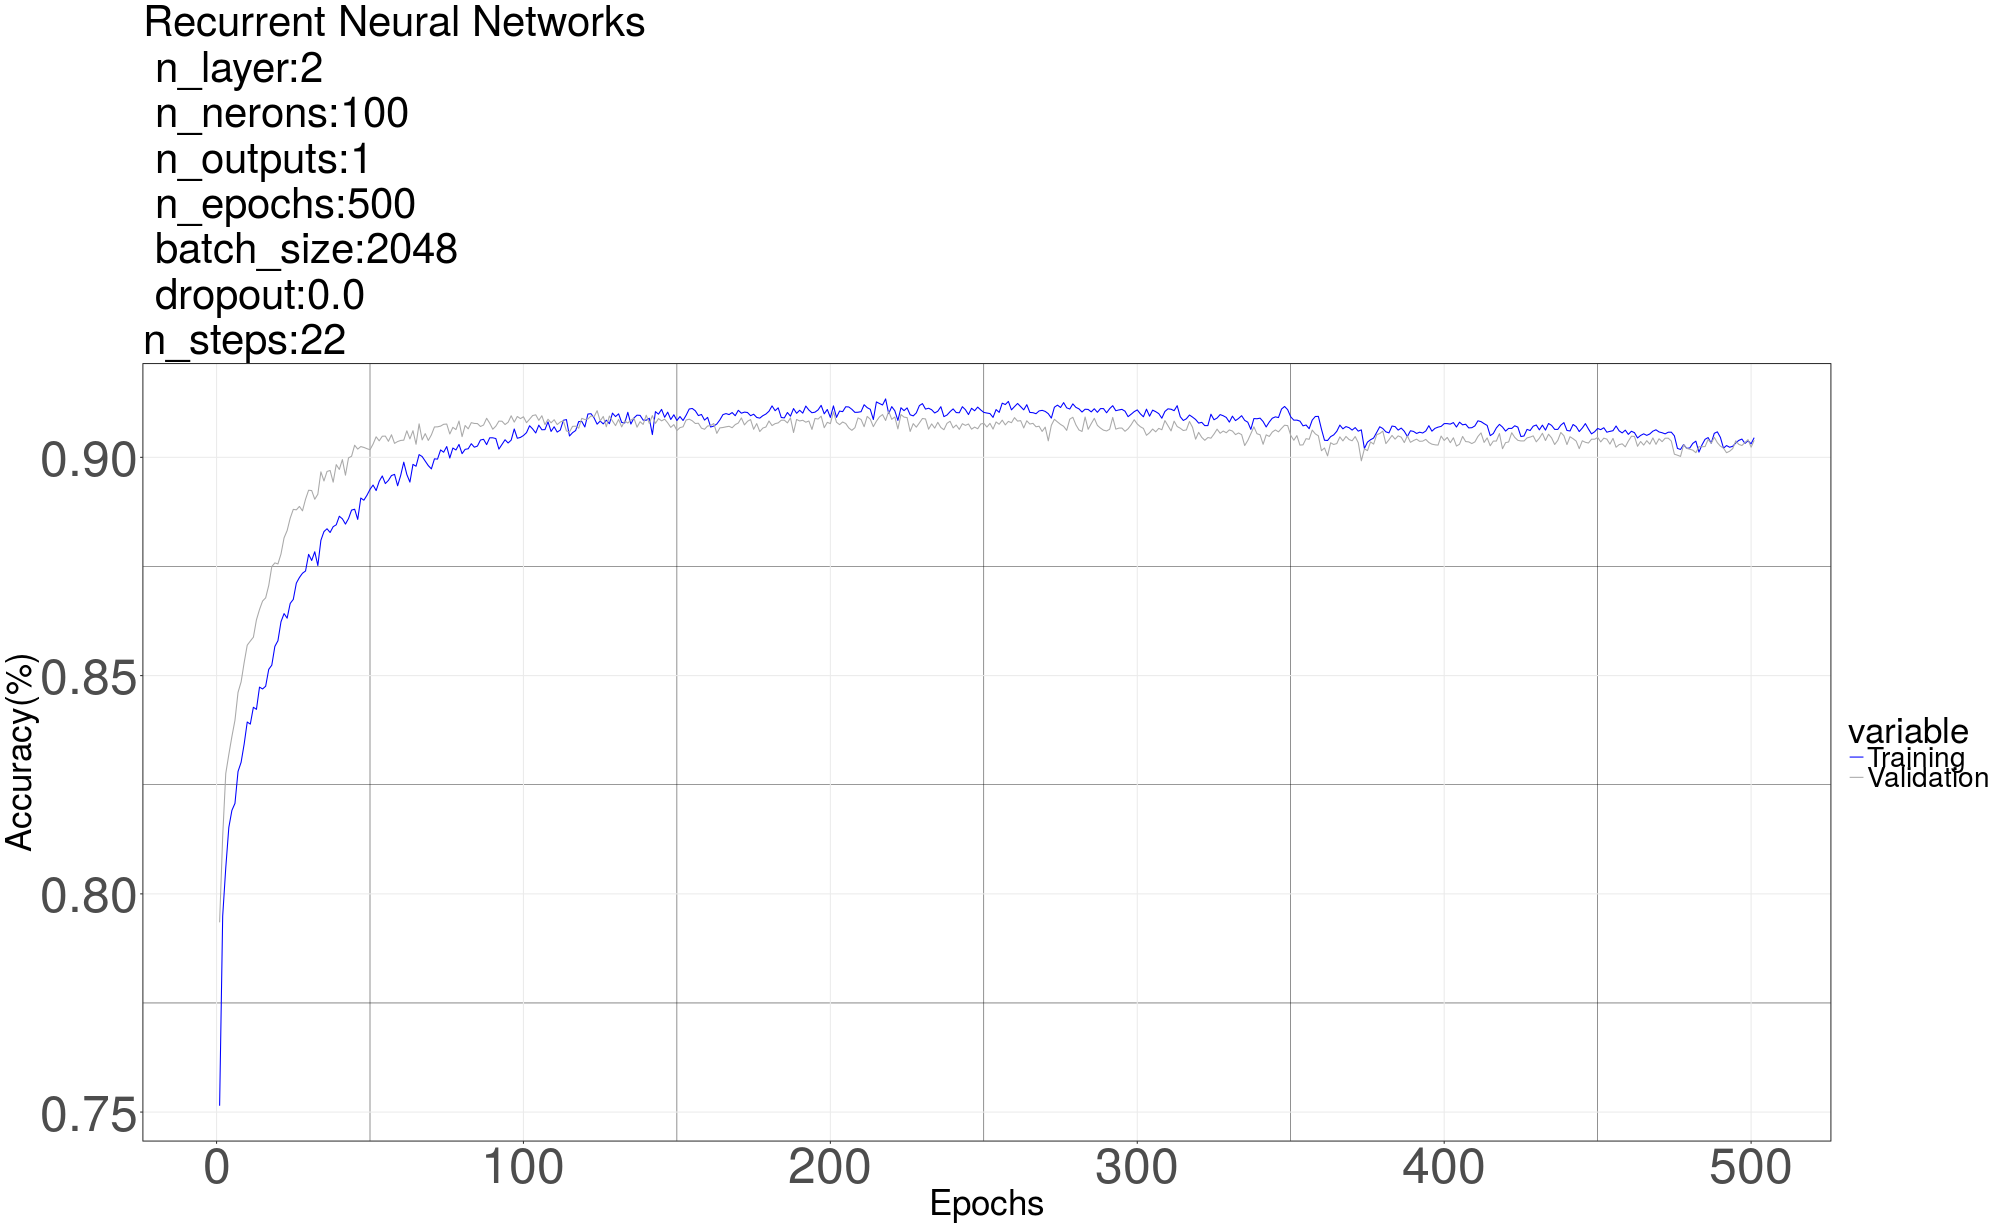
\includegraphics[width=1.0\textwidth]{RNN_3.png}
\caption{\label{fig:RNN_3}Results of Recurrent Neural Network on Training and Validation set. Title contains information about configuration of the network.}
\end{figure}

\begin{figure}  
\centering
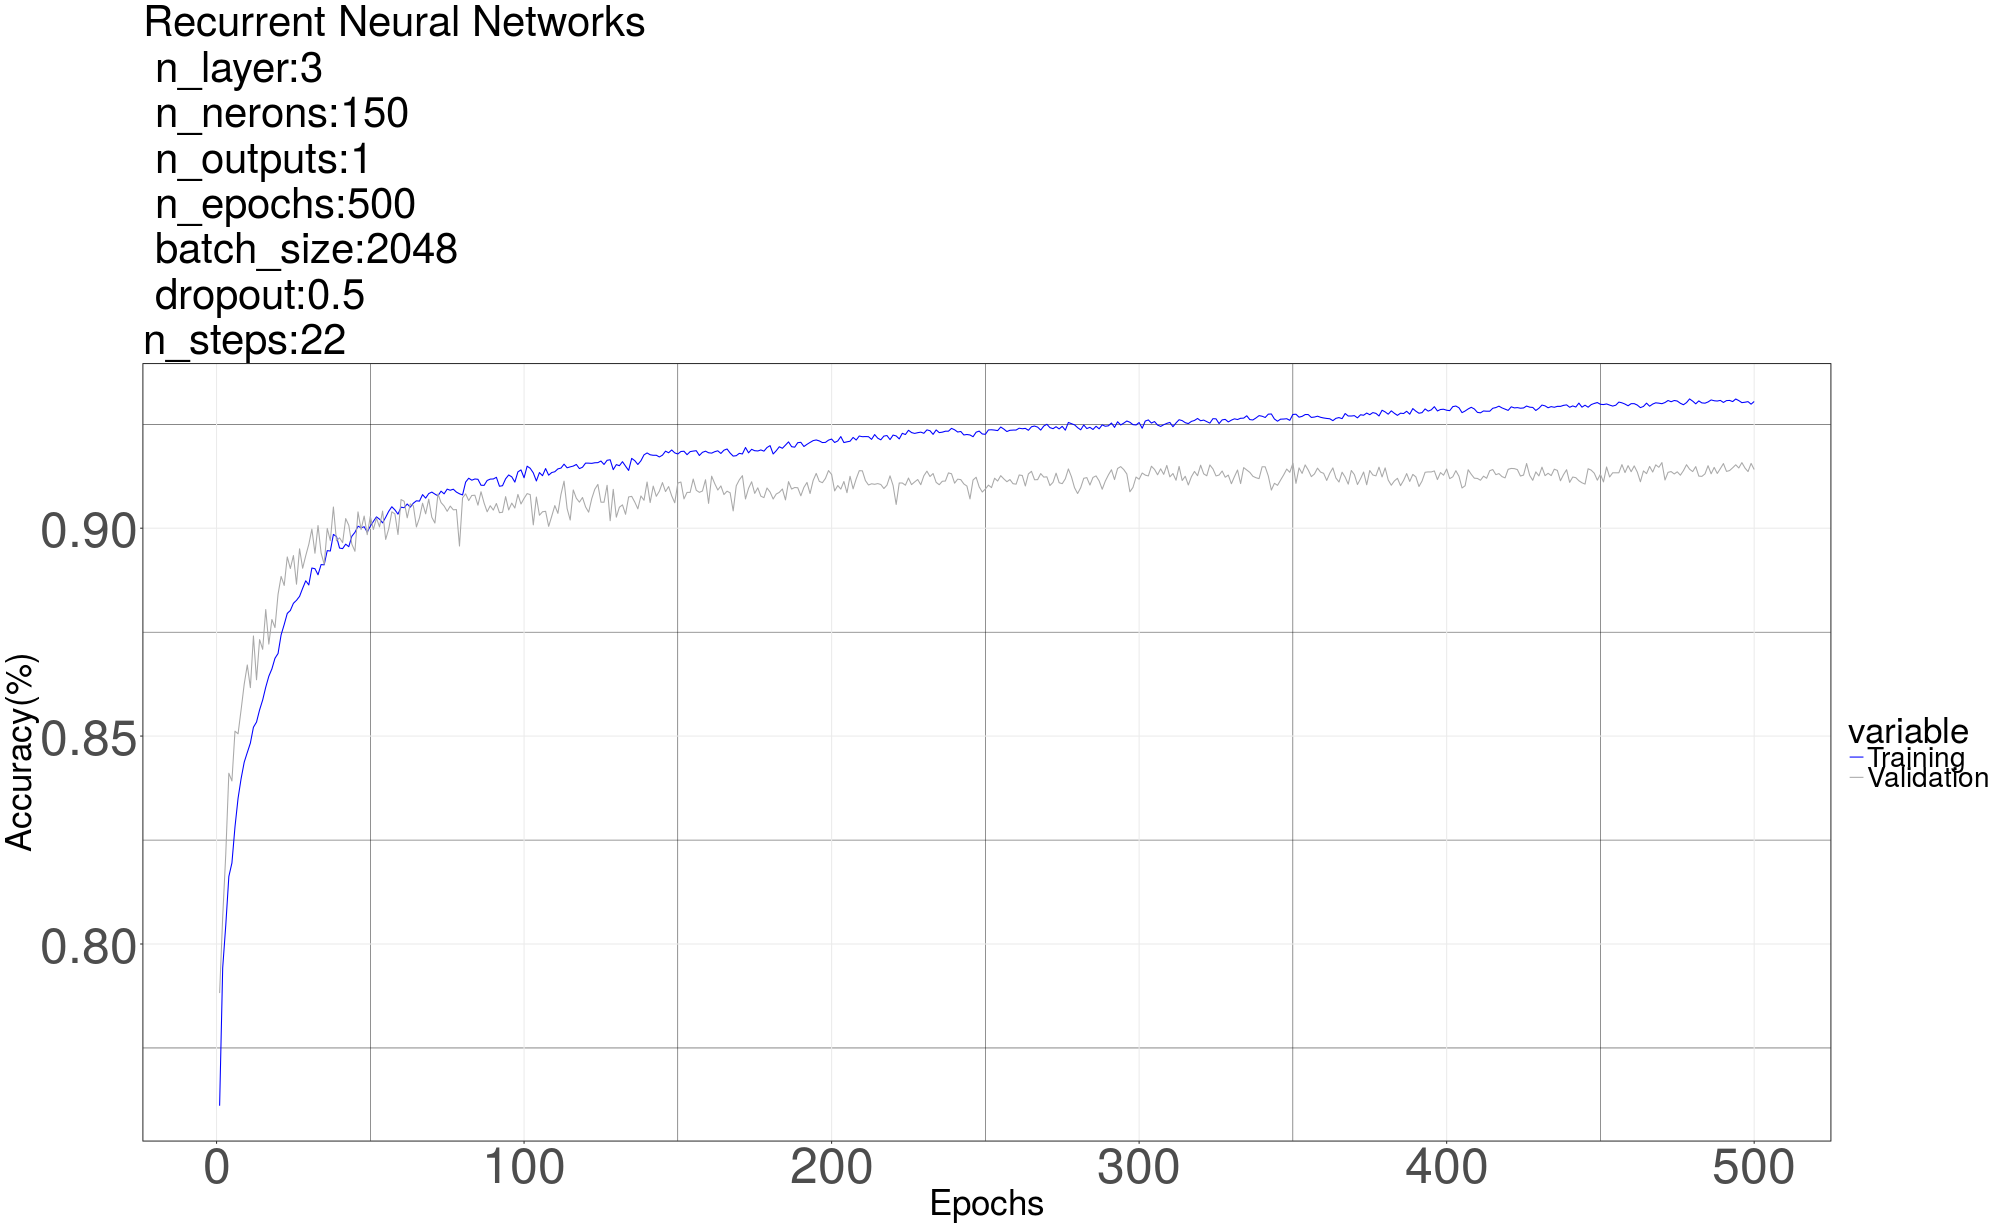
\includegraphics[width=1.0\textwidth]{RNN_4.png}
\caption{\label{fig:RNN_4}Results of Recurrent Neural Network on Training and Validation set. Title contains information about configuration of the network.}
\end{figure}


\begin{figure}  
\centering
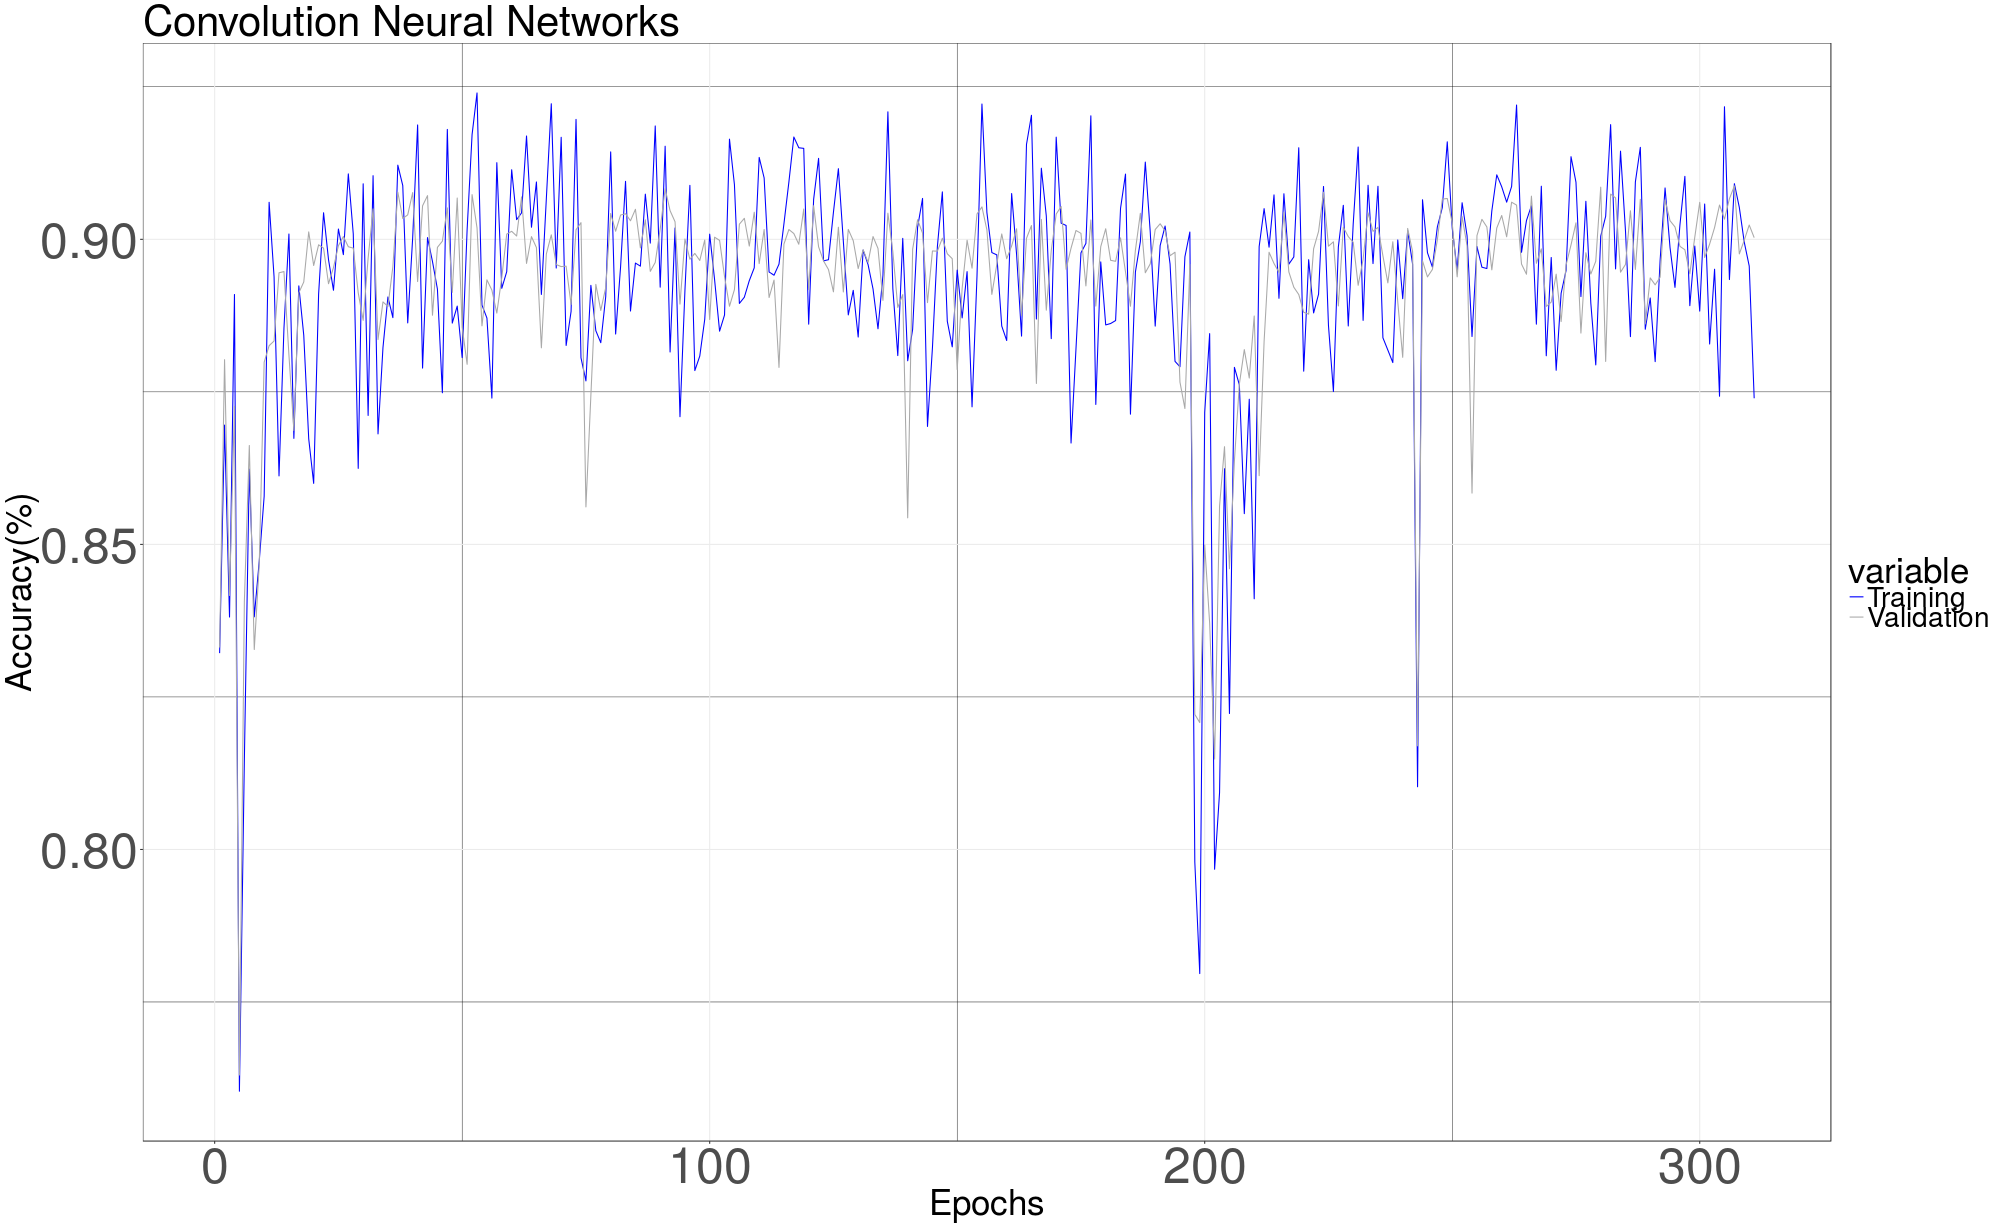
\includegraphics[width=1.0\textwidth]{CNN_1.png}
\caption{\label{fig:CNN_1}Results of Convolution Neural Network on Training and Validation set. Title contains information about configuration of the network.}
\end{figure}



\begin{figure}  
\centering
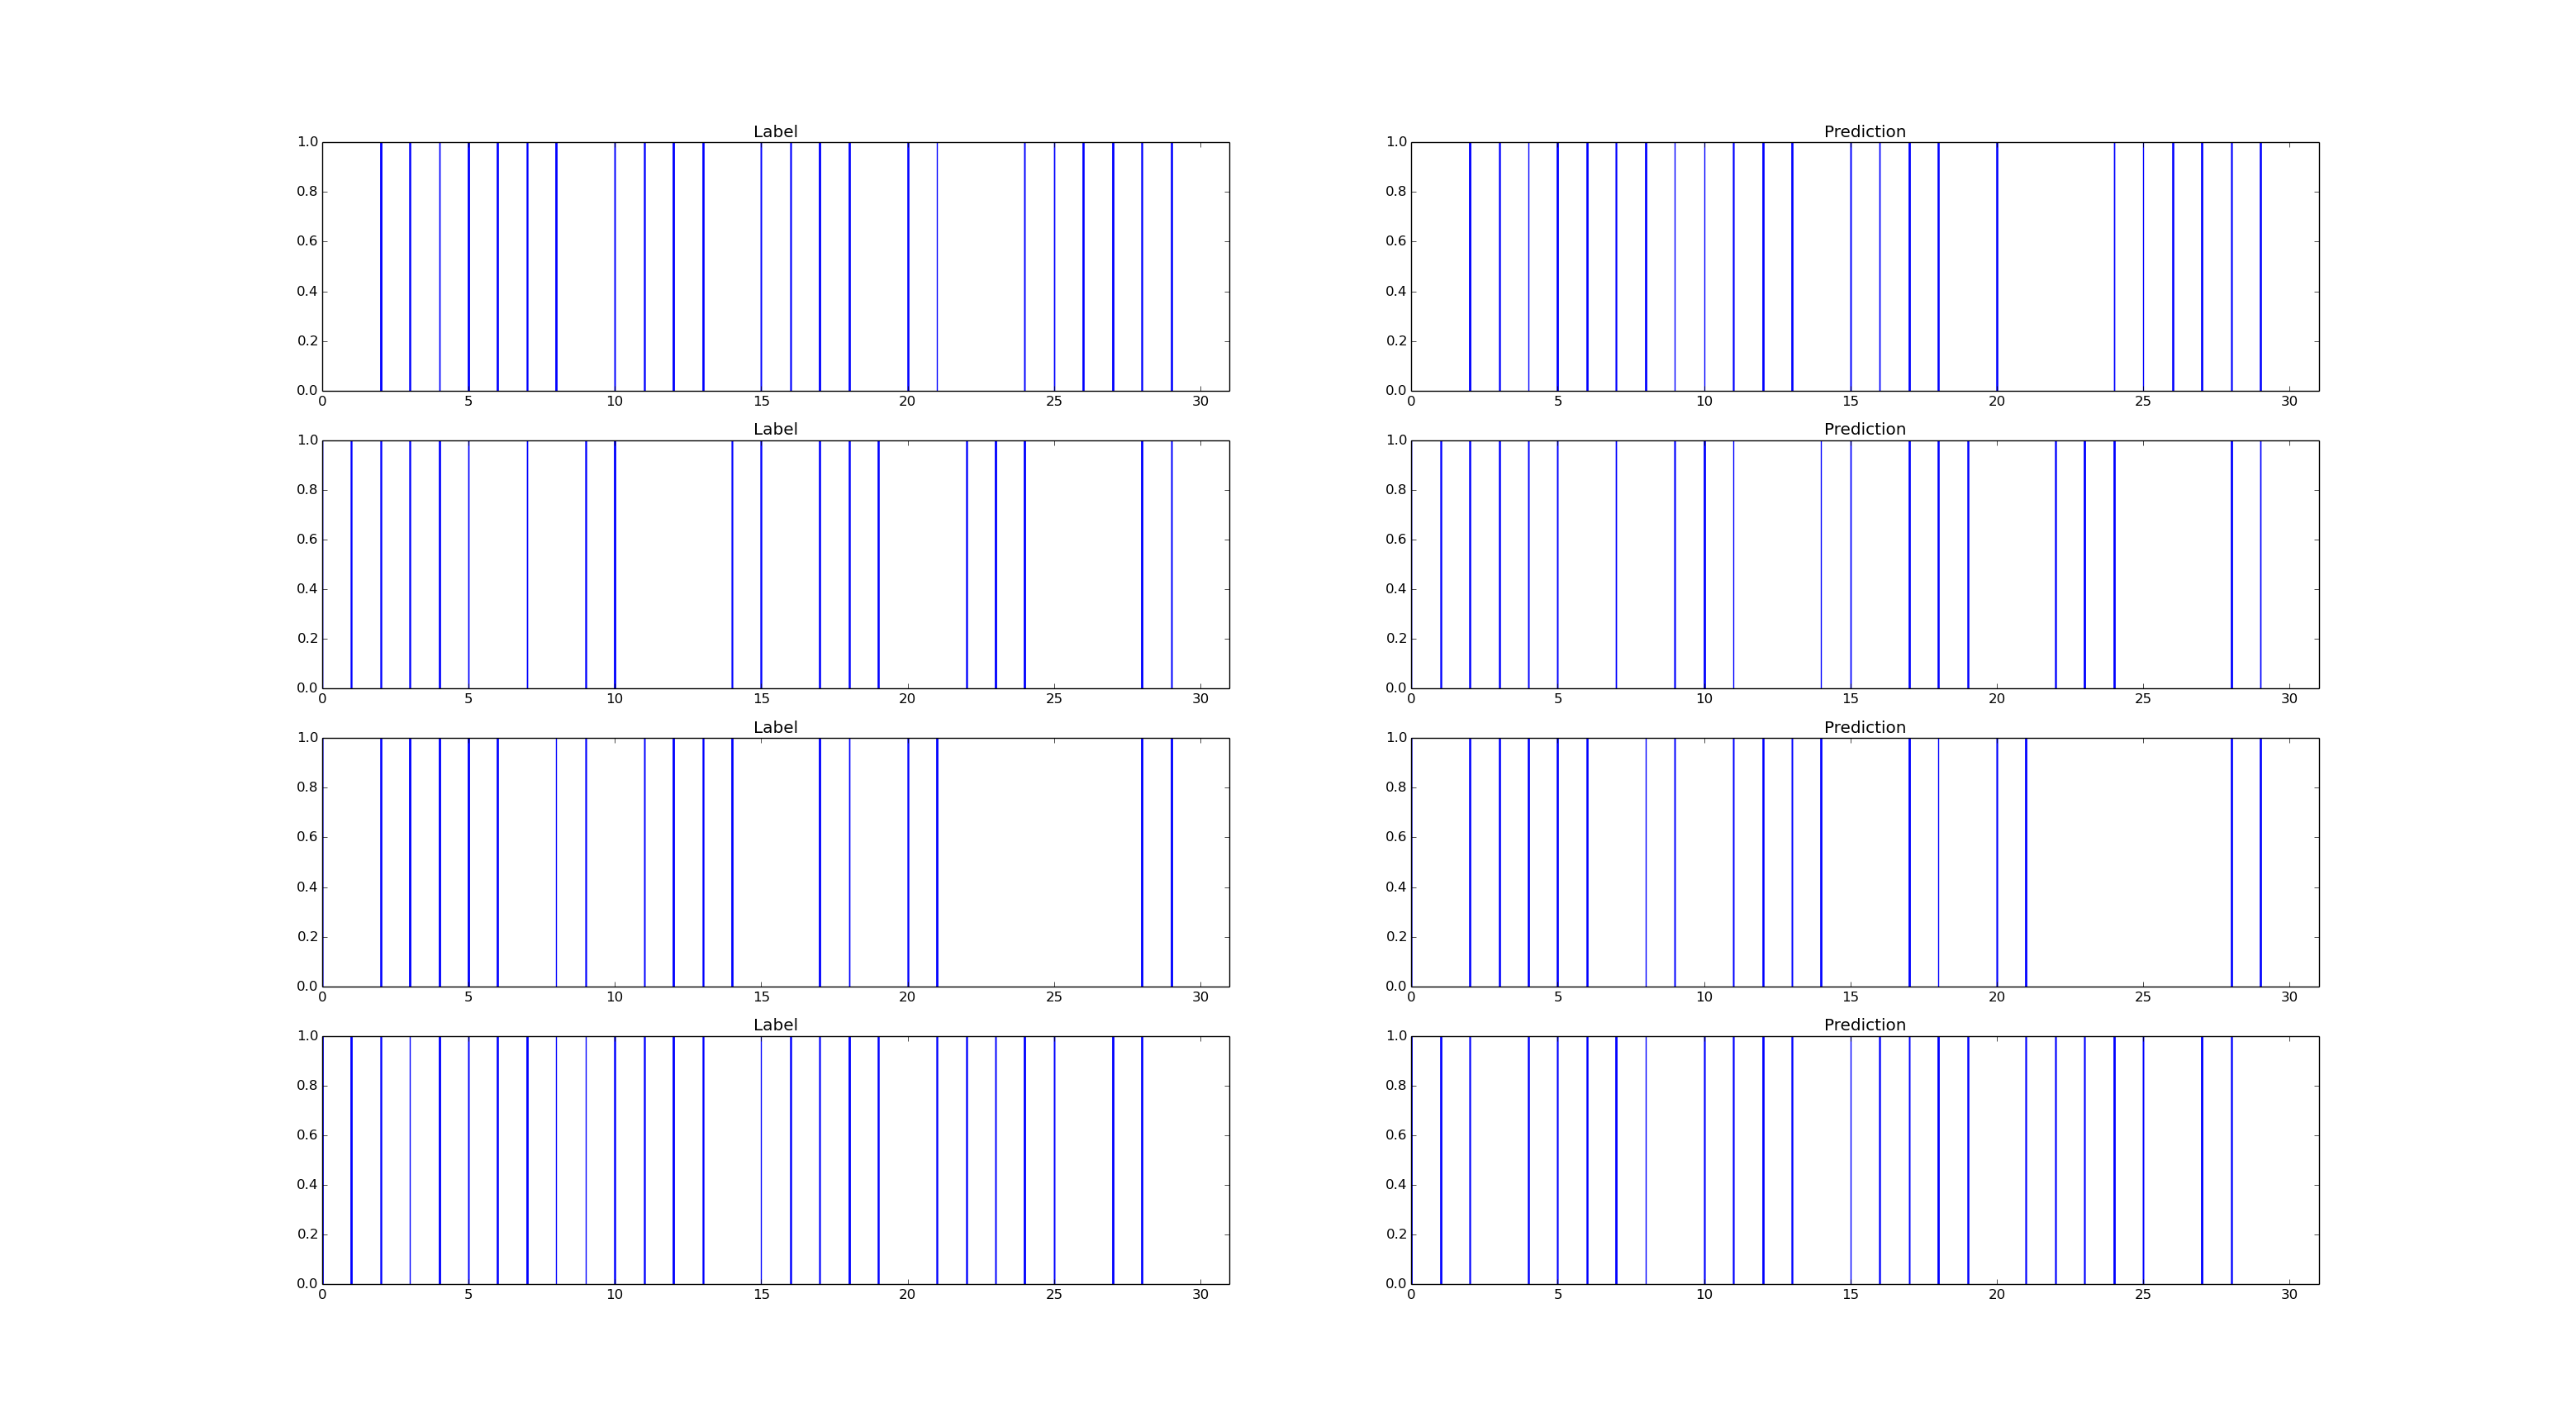
\includegraphics[width=1.0\textwidth]{CompareLabelNPrediction.png}
\caption{\label{fig:comapre}Compare Predicted with given Label.}
\end{figure}




\bibliographystyle{alpha}
\bibliography{sample}

\end{document}